\section{The Quantum Channel - System Outline}
\label{sec:outline}

In this section, an outlined description of the basic functionality of the complete quantum channel system will be given. The interaction of system components will be described in different modes of operation that can be configured for the quantum channel.

\subsection{The EPR Source}
\label{subsec:outline_source}

The \textbf{source} generates photon pairs with a specific photon rate. For each generated photon pair, it generates two events: the first one is sent to \textbf{detector alice}, the second one to the \textbf{fiber}. As can be seen in Figure \ref{fig:quantum_channel}, the event which is sent to the \textbf{fiber} is assigned \texttt{SUBNORMAL} event priority. Priority changes for events are always indicated with fine dashed lines and rectangles containing the priority names. These priority changes are always only valid in the direction of signal flow, not backwards. If no priority assignments are made to an event, \texttt{NORMAL} event priority is assumed as default.
The reason why \texttt{SUBNORMAL} priority is assigned to the event sent to the \textbf{fiber} is that \textbf{detector alice} should process the photon pair generation event first, because in \textit{sync mode} this will lead to the generation of a sync pulse, which is also transmitted over the \textbf{fiber} as a \texttt{SYNC\_PULSE} event with \texttt{NORMAL} event priority, so that (in the case that an idealised simulation is performed with no delay times configured for delay fibers) it will reach \textbf{detector bob} first before the photon pair generation event with \texttt{SUBNORMAL} event priority arrives. This behaviour is required because the sync pulse should trigger \textbf{detector bob} that it becomes ready to receive a photon event.

\subsection{The Transmission Fiber}
\label{subsec:outline_fiber}

The transmission fiber with its components is shown in Figure \ref{fig:outline_fiber}. 

\begin{figure}[h]
\centering
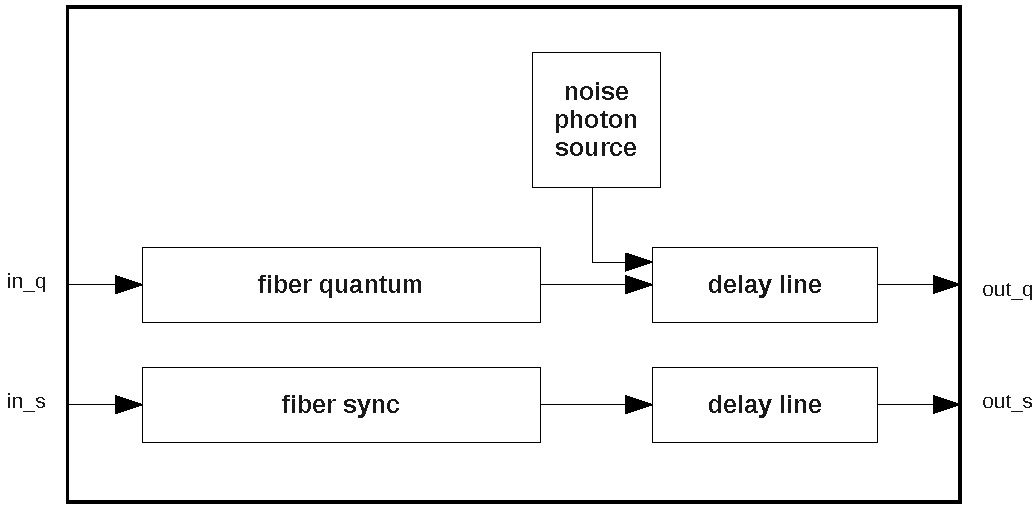
\includegraphics[scale=0.65]{drawings/fiber.pdf}
\caption{The transmission fiber}
\label{fig:outline_fiber}
\end{figure}

The transmission of photons is modelled to occur over a quantum transmission fiber (\textbf{fiber quantum}) and the transmission of the sync pulse over a sync pulse transmission fiber (\textbf{fiber sync}), although in reality they are both transmitted over the same fiber but at another wavelength using wavelength-division multiplexing (WDM) as already mentioned in section \ref{sec:overview}. There are also two \textbf{delay line}s that allow to model delay times between the photons and the sync pulse so that the photons arrive at Bob's detector later or earlier than the sync pulse. Also there is shown a \textbf{noise photon source} that is used for simulating stray light photons interspersed into the quantum transmission fiber. Photons generated by the \textbf{noise photon source} are stored as \texttt{photon\_pair} objects (see section \ref{subsec:concepts_photons}) where \texttt{m\_eStateA} is set to \texttt{ABSORBED} and \texttt{m\_eStateB} is set to \texttt{NONPOLARIZED}.

\subsection{Detector at Alice's Side}
\label{subsec:outline_detector_alice}

The different components of the detector at Alice's side are shown in Figure \ref{fig:outline_detector_alice} and will now be briefly described.

\begin{figure}[h]
\centering
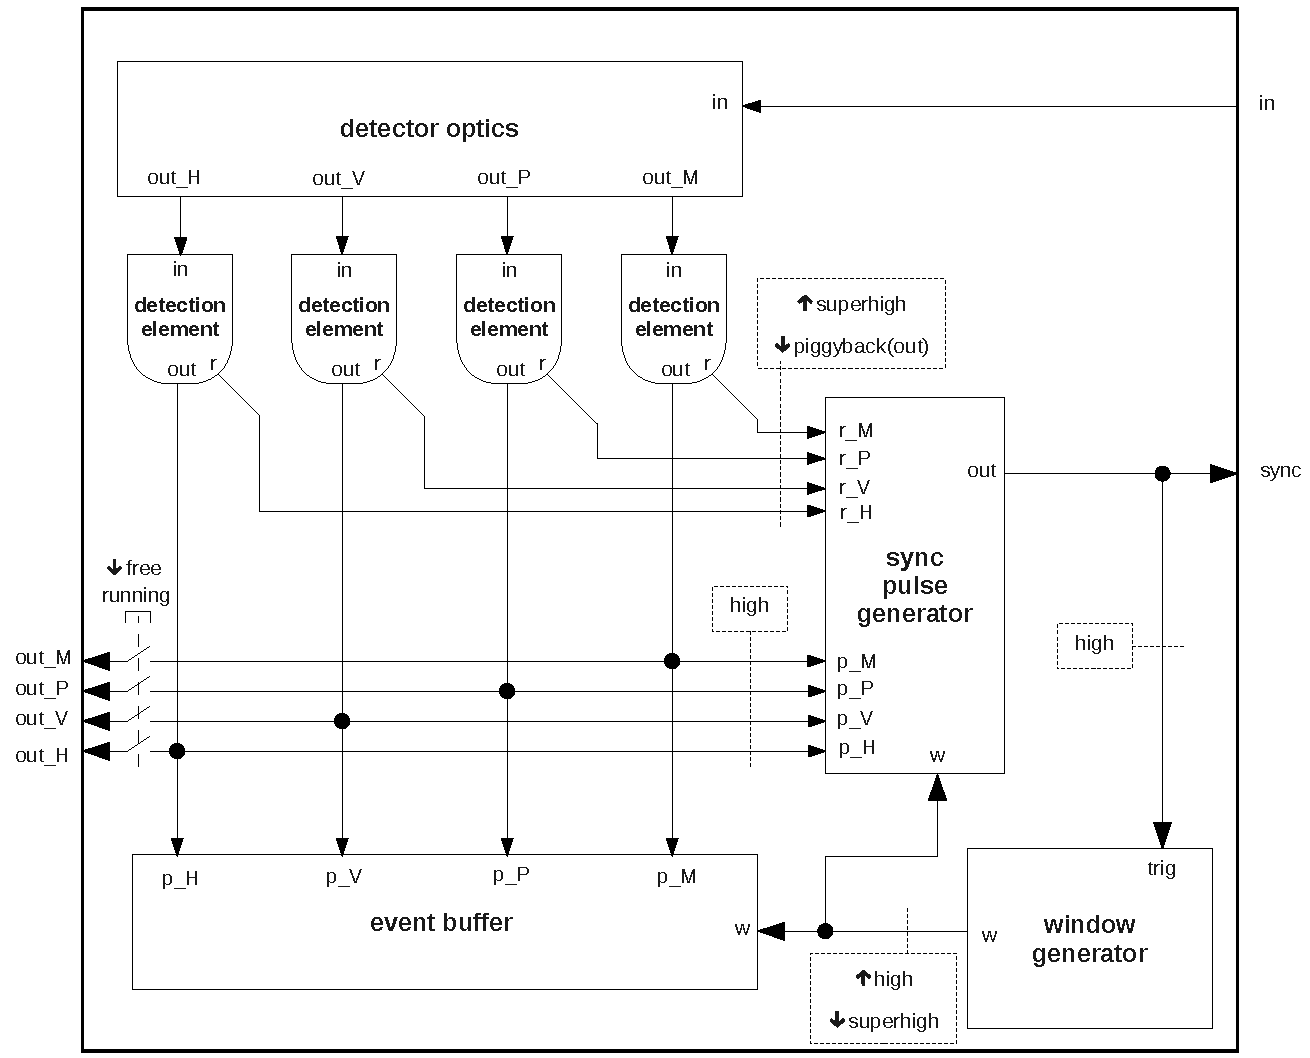
\includegraphics[scale=0.65]{drawings/detector_alice.pdf}
\caption{The detector at Alice's side}
\label{fig:outline_detector_alice}
\end{figure}

The \textbf{detector optics} component's purpose is to model optical components in the BB84 detector such as polarising and non-polarising beam splitters. When it receives an incident \texttt{photon} event, it makes random choices to decide to which of the four \textbf{detection element}s an incoming \texttt{photon} event will be sent, where the probabilities of the photon being forwarded to the specific \textbf{detection element}s are chosen depending on the incoming photon's polarisation in such a way that they reproduce the behaviour of the modelled BB84 detector.

The \textbf{detection element}s represent the four single photon detectors. Whenever they receive and detect a photon they generate an electrical \texttt{pulse} event. What happens next depends on which detection mode has been configured. There are four different modes available for Alice's detector:

\begin{itemize}

\item \textit{free running mode}: The electrical \texttt{pulse} events generated by the \textbf{detection element}s are forwarded by \textbf{detector alice} to \textbf{channel} and further to the \textbf{TTM} module (see Figure \ref{fig:quantum_channel}) which records the received events to a logging file named \texttt{TTM.log}.

\item \textit{sync mode}: The electrical \texttt{pulse} events generated by the \textbf{detection element}s are sent to the \textbf{sync pulse generator} and to the \textbf{event buffer}. As can be seen in Figure \ref{fig:outline_detector_alice}, the \texttt{pulse} event sent to the sync pulse generator is assigned \texttt{high} priority so that is arrives before the \textbf{event buffer} receives the \texttt{pulse} event. A second output each \textbf{detection element} provides is the `ready'' output (labelled with ``r'') that informs the \textbf{sync pulse generator} if the \textbf{detection element}s are in ready or down state. If a ``down time'' parameter has been configured for the \textbf{detection element}s, this means that whenever they receive a photon, they go into down state, and after some down time has passed, they go back into ready state. 
The beginning of a down period is indicated to the \textbf{sync pulse generator} by a flag transmitted together with the output \texttt{pulse} event - this is the reason why a downward arrow with the text ``piggyback(out)'' is shown in Figure \ref{fig:outline_detector_alice}. In this case, it exceptionally does not indicate the priority of a newly generated event but signifies that the information that a falling edge at the ``ready'' output occurred is transported piggyback by a flag included in the \texttt{pulse} output event. In the other case, however, that a rising edge occurs at the ``ready'' output (after the down time is over) an extra event of type \texttt{down\_end} with \texttt{superhigh} priority is generated and sent to the \textbf{sync pulse generator}.

Whenever the \textbf{sync pulse generator} receives a \texttt{pulse} event from a \textbf{detection element}, it checks if the \textbf{window generator} is currently ready (it has finished generating its last window, if one was triggered), and if it is, the \textbf{sync pulse generator} generates a \texttt{SYNC\_PULSE} event with \texttt{high} priority that is on the one hand forwarded by \textbf{detector alice} to \textbf{channel} and then further to \textbf{fiber}, and on the other hand it triggers the \textbf{window generator} to generate a new window of specified duration.

The rising edge of the \textbf{window generator}'s output signal (= the beginning of the new window) is signalled as a \texttt{high} priority event of type \texttt{WINDOW\_START} to the \textbf{event buffer}. The \textbf{event buffer} in turn hereupon clears its 4-bit-wide event latch and opens it to receive and store \texttt{pulse} events coming from the \textbf{detection element}s. Whenever further some \texttt{pulse} event coming from a \textbf{detection element} is send to the \textbf{event buffer} while its event latch is open, it stores a ``1'' for the bit in the event latch corresponding to the respective \textbf{detection element}. 

This now shows the reason why \texttt{high} priority events are necessary for the \texttt{pulse} event send from the \textbf{detection element}s to the \textbf{sync pulse generator} and from the \textbf{sync pulse generator} to the \textbf{window generator} as well as for the \texttt{WINDOW\_START} event sent to the \textbf{event buffer}: It must be ensured that a \texttt{pulse} event coming from a \textbf{detection element} that triggers a new window can open the \textbf{event buffer}s event latch first before the \texttt{pulse} event itself is sent to the \texttt{event buffer} so that it gets stored in the event latch. 

After some time, the \textbf{window generator} closes its window and signals the falling edge of the window output signal by sending a \texttt{WINDOW\_END} event of \texttt{superhigh} priority to the \textbf{event buffer} and the \textbf{sync pulse generator}, which causes the \textbf{event buffer} to close its event latch and write its contents to a key buffer, and also informs the \textbf{sync pulse generator} that the \textbf{window generator} is now ready to generate a new window. The \texttt{superhigh} priority is used for the \texttt{WINDOW\_END} event because in the case that at the same time a new \texttt{pulse} event comes from a \textbf{detection element}, it shall be ensured that at first the \textbf{event buffer} and the \textbf{sync pulse generator} are informed that the previous window has been closed.

\item \textit{sync mode - wait for sync initiator to be ready}: The behaviour of \textbf{detector alice} is almost the same as in \textit{sync mode}, with the only difference that whenever the \textbf{sync pulse generator} generates a sync pulse, it remembers which of the four \textbf{detection element}s was the initiator of the sync pulse, and in the case that the initiating \textbf{detection element} goes into down state after sending the \texttt{pulse} event, the \textbf{sync pulse generator} does not generate new sync pulses until the initiating \textbf{detection element} goes back into ready state.

\item \textit{sync mode - wait for all detection elements to be ready}: The behaviour of \textbf{detector alice} is almost the same as in \textit{sync mode}, with the only difference that the \textbf{sync pulse generator} does only generate a sync pulse if all \textbf{detection element}s are in ready state (none of them is down).

\end{itemize}

\subsection{Detector at Bob's Side}
\label{subsec:outline_detector_bob}

The detector at Bob's side with its components is shown in Figure \ref{fig:outline_detector_bob}. It looks very similar to that at Alice's side, with the difference that instead of a \textbf{sync pulse generator} it contains a \textbf{sync pulse receiver}, and the \textbf{detection element}s, the \textbf{window generator} and the \textbf{event buffer} have some extra input and output signals (bad, bad\_out).

\begin{figure}[h]
\centering
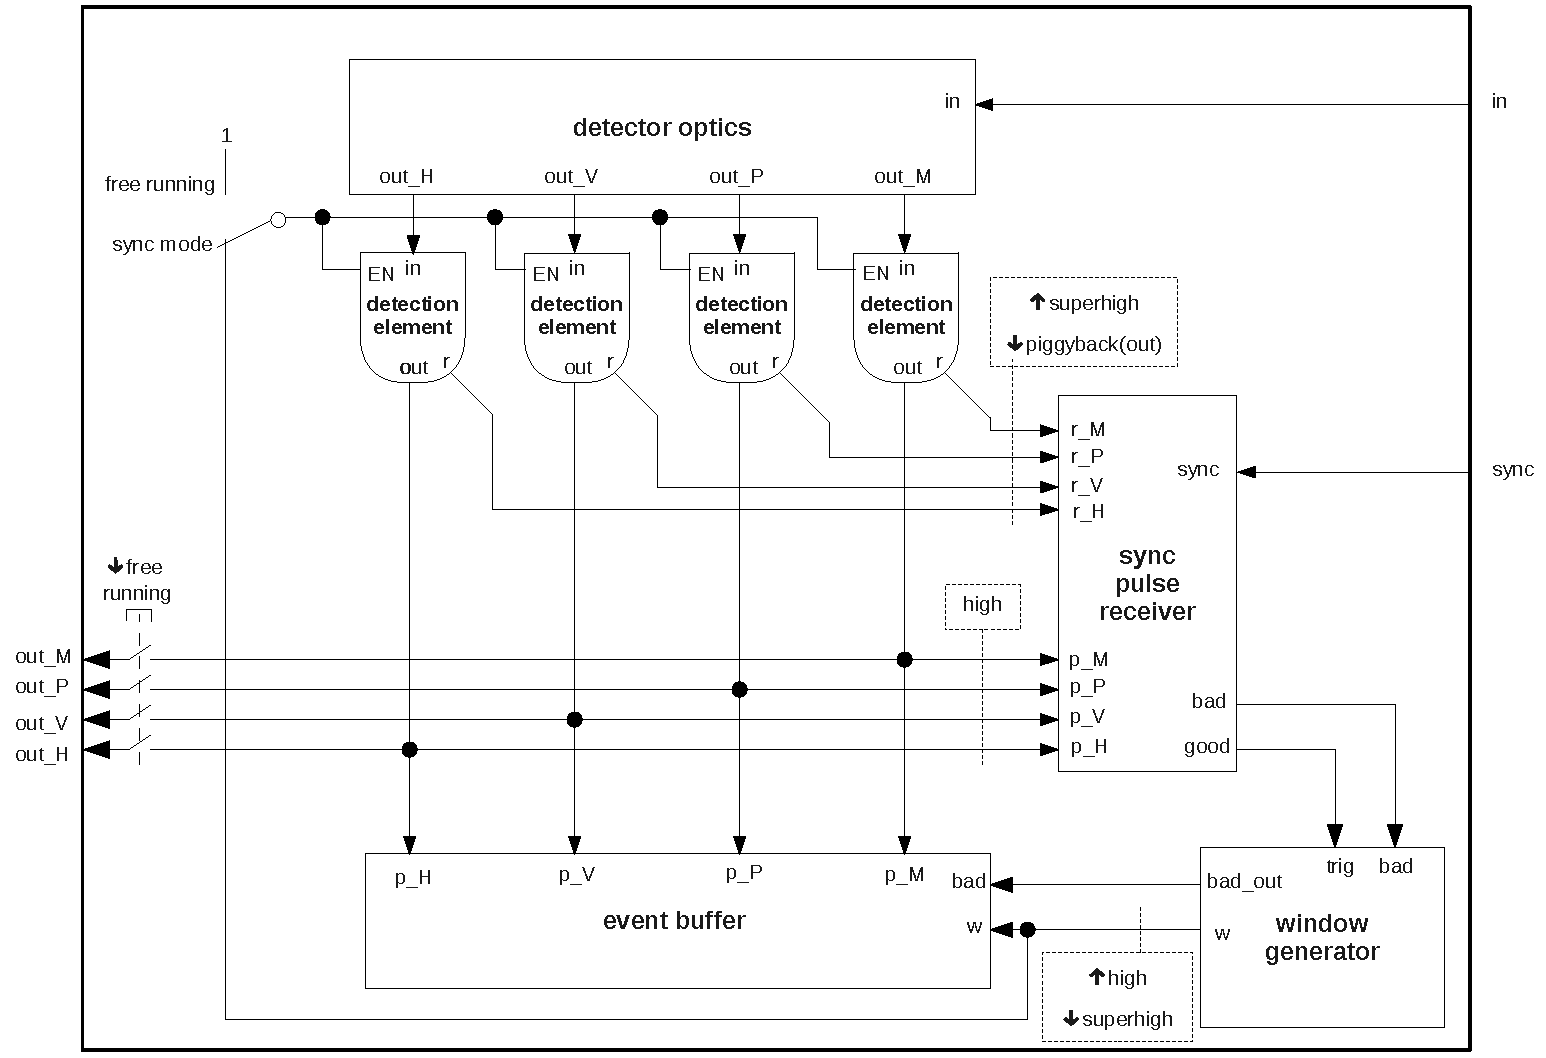
\includegraphics[scale=0.65]{drawings/detector_bob.pdf}
\caption{The detector at Bob's side}
\label{fig:outline_detector_bob}
\end{figure}

The behaviour of many parts of \textbf{detector bob} is the same as for \textbf{detector alice} - therefore, only the differences are described now. There are three possible operation modes for \textbf{detector bob}:

\begin{itemize}

\item \textit{free running mode}: In this mode, \textbf{detector bob} behaves exactly in the same way as \textbf{detector alice} does. Additionally it must be noted that in this mode, the delay time for the delay line connected to the output of the quantum transmission fiber (see Figure \ref{fig:outline_fiber}) is set to zero, so that when all system components parameters are configured for the ideal case, the same detection times are recorded by the TTM for the two photons (travelling to Alice and Bob) belonging to one entangled photon pair.

\item \textit{sync mode}: Whenever the \textbf{sync pulse receiver} receives a \texttt{SYNC\_PULSE} event (that originally came from \textbf{detector alice}'s \textbf{sync pulse generator} and travelled over the \textbf{fiber}) it triggers the window generator by sending a \texttt{SYNC\_PULSE} event to it. The \textbf{window generator} in turn sends a \texttt{WINDOW\_START} event to the \textbf{event buffer}. In the case that there was already a window opened by the \textbf{window generator} and has not been closed before, the \textbf{window generator} newly calculates when the \texttt{WINDOW\_END} event should occur (according to the configured window duration). 

The \textbf{detection element}s operate in a ``gated'' mode - they are only enabled to receive photons when the \textbf{window generator}'s output is currently in high state (which means that a window is currently open).

The \textbf{event buffer} operates in the same way is in \textbf{detector alice}, but with the additional feature that when it receives a \texttt{WINDOW\_START} event when its event latch is already open (no \texttt{WINDOW\_END} event came after the previous \texttt{WINDOW\_START} event), it writes the current contents of the event latch to the key buffer, clears the event latch and the event latch remains in opened state.

\item \textit{sync mode - wait for all detection elements to be ready}: The \textbf{detector bob} operates similarly as in \textit{sync mode} but with some differences and enhancements: In the case that the \textbf{sync pulse receiver} receives a \texttt{SYNC\_PULSE} event while not all \textbf{detection element}s are in ready state, it sends a \texttt{SYNC\_PULSE\_BAD} event instead of a \texttt{SYNC\_PULSE} event to the \textbf{window generator}. 

When the \textbf{window generator} receives the \texttt{SYNC\_PULSE\_BAD} event, how it acts depends on its current state: If no window is open currently, the \textbf{window generator} sends a \texttt{SYNC\_PULSE\_BAD} event to the \textbf{event buffer}. If a window is currently open, however, the \textbf{window generator} closes the active window and sends a \texttt{window\_end\_bad} event to the \textbf{event buffer}.

The \textbf{event buffer}, when it receives a \texttt{SYNC\_PULSE\_BAD} event, writes a zero entry to the key buffer. When the \textbf{event buffer} receives a \texttt{window\_end\_bad} event, it first closes its event latch and writes the current contents of the event latch to the key buffer, then it additionally writes a zero entry to the key buffer.

\end{itemize}
